\lettrine[findent=0.4em, nindent=0em]{\textbf{P}}{robabilistic analysis} of
electronic systems is an extensive and diverse area, which is expanding with an
accelerating pace. The rapid growth is instigated by the fact that electronic
systems naturally become more sophisticated and refined, and that they penetrate
deeper into everyday life. Therefore, the impact of uncertainty inevitably
becomes more prominent and entails more severe consequences, necessitating an
adequate treatment. Consequently, the designer of an electronic system is
obliged to account for the presence of uncertainty in order to produce an
efficient and reliable product.

In order to account for uncertainty, one has to quantify it first. In this
setting, one is usually interested in a quantity---referred to as the quantity
of interest---whose complete knowledge would be highly profitable for the design
at hand but cannot be attained since the quantity depends on a number of
parameters that are inherently uncertain at design time. Consider, for instance,
the maximum temperature of a system running a number of tasks whose execution
times are random.

Uncertainty quantification is a broad umbrella. The corresponding techniques can
deliver radically different pieces of information about the quantity of
interest. In this paper, we are interested in probability distributions rather
than, for instance, corner cases. Designing for the worst case leads often to a
poor solution as the system under consideration might easily end up being too
conservative, overdesigned \cite{quinton2012}.

When it comes to the estimation of probability distributions and to uncertainty
quantification in general, sampling methods are of great use. The classical
Monte Carlo (\up{MC}) sampling, quasi-\up{MC} sampling, and Latin hypercube
sampling are examples of such methods \cite{asmussen2007}. Compared to other
techniques for probabilistic analysis, these methods are straightforward to
apply. The system at hand is treated as a completely opaque object, and one only
has to evaluate this object a number of times in order to start to draw
conclusions about the system's behavior. Consider, for instance, \up{MC}
sampling, which is arguably the most famous and versatile approach to
uncertainty quantification. The technique was introduced in the middle of the
twentieth century and, since then, has expanded into a rich family of methods
that have had a tremendous impact both in academia and in terms of industrial
breakthroughs \cite{asmussen2007}.

The major problem with sampling techniques, however, is in sampling: one should
be able to obtain sufficient many realizations of the quantity of interest in
order to accurately estimate the needed statistics about that quantity
\cite{diaz-emparanza2002}. The main concerns in this context are: How much does
it cost in terms of time and other resources to obtain one sample? How many
samples do we need? How many can we afford? When the subject under analysis is
expensive to evaluate, sampling methods are rendered slow and often unfeasible.

We propose a design-time system-level framework for the analysis of electronic
systems that are dependent on uncertain parameters. Similar to sampling methods,
our technique treats the system at hand as a ``black box'' and, therefore, is
straightforward to apply since no handcrafting is required, and existing codes
need no change. Consequently, the quantities of interest that the framework is
able to tackle are diverse. Examples include those quantities concerned with
timing-, power-, and temperature-related characteristics of elaborate
applications running on heterogeneous multiprocessor platforms.

In contrast to sampling methods, our technique explores and exploits the nature
of the problem---that is, the way the quantity of interest depends on the
uncertain parameters---by exercising the aforementioned ``black box'' at a set
of points chosen adaptively. The adaptivity that our framework leverages is
hybrid \cite{jakeman2012}: it tries to pick up both global (that is, on the
level of entire dimensions \cite{klimke2006}) and, more importantly, local (that
is, on the level on individual points \cite{ma2009}) variations. This means that
the framework is able to benefit from many particularities that might be present
in the stochastic space, that is, the space of the uncertain parameters. The
adaptivity is the capital feature of our technique, and we would like to
elaborate on it now. To this end, let us first make one general observation.

The uncertainties present in electronic systems originate from both the physical
world and the computer world. An example of a physical source of uncertainty is
process variation \cite{srivastava2005}, which is a side effect of contemporary
fabrication processes. Process variation has been central for many lines of
research \cite{bhardwaj2008, juan2012, lee2013, ukhov2014, ukhov2015}. An
example of a digital source of uncertainty (the computer world) is workload. To
elaborate, the characteristics of the codes running on modern devices change
from one activation to another depending on the environment and input data. This
source of uncertainty has not been deprived of attention either, especially in
the real-time community \cite{quinton2012, diaz2002, santinelli2011,
tanasa2015}. Regardless of the origin, such phenomena as the ones mentioned
above render the behavior of an electronic system nondeterministic to the
designer, and accounting for them is highly beneficial if not essential.

\begin{figure}
  \centering
  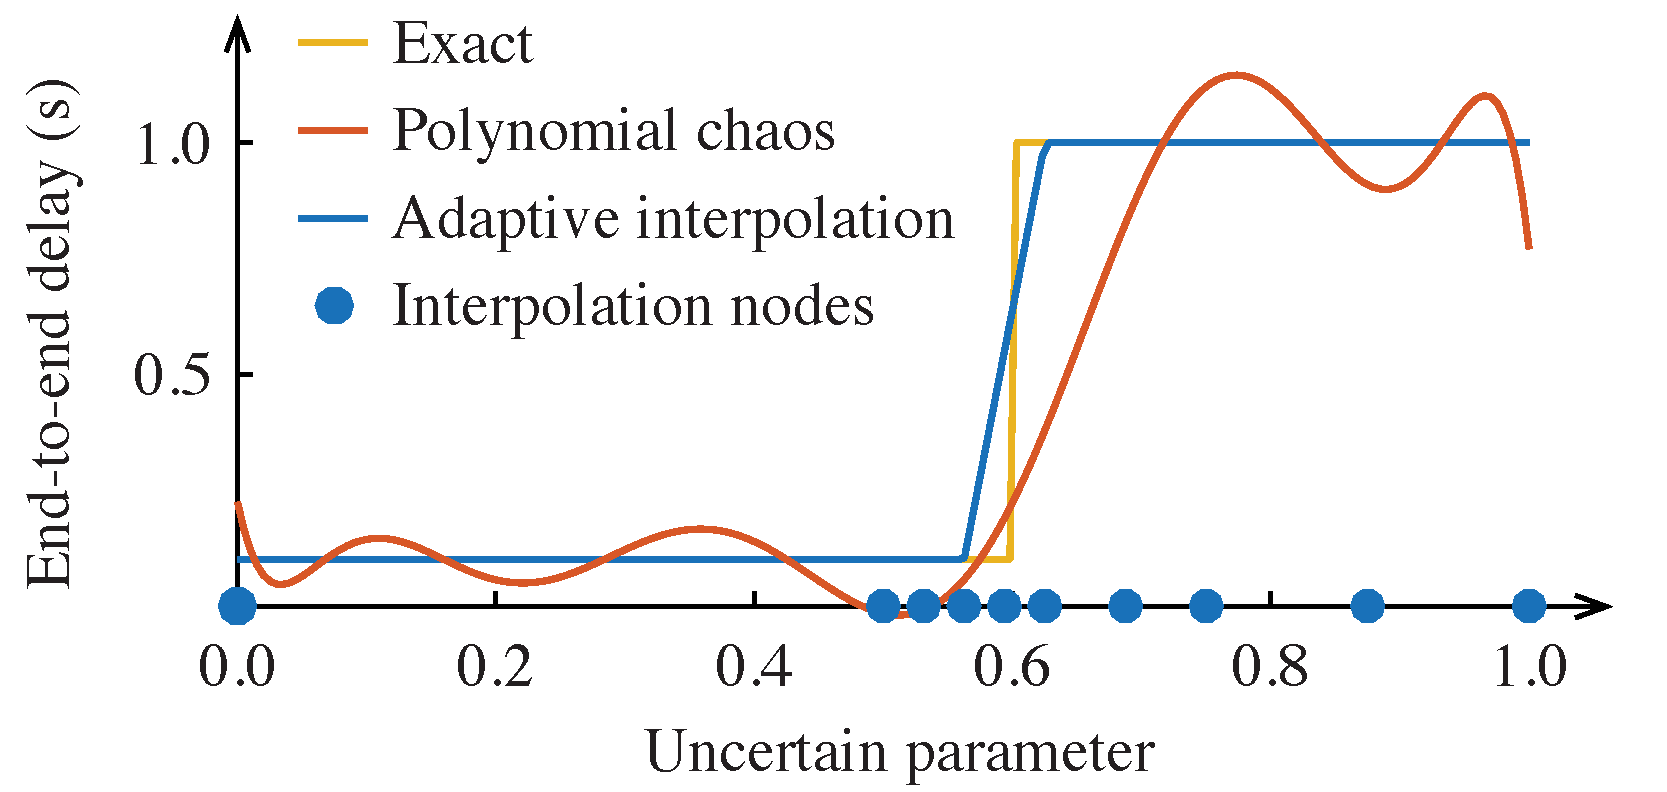
\includegraphics[width=1.0\columnwidth]{include/assets/figures/motivation.pdf}
  \caption{
    A motivational example.
  }
  \flab{motivation}
\end{figure}

Due to its nature, the variability coming from the physical world is typically
smooth, well behaved. In such cases, uncertainty quantification based on
polynomial chaos (\up{PC}) expansions \cite{xiu2010} and other approximation
techniques making use of global polynomials generally work well, as in
\cite{bhardwaj2008, lee2013, ukhov2014, ukhov2015}. On the other hand, the
variability coming from the computer world has often steep gradients and favors
nondifferentiability and even discontinuity. In such cases, \up{PC} expansions
and similar techniques fail: they require extremely many evaluations of the
quantity of interest in order to deliver an acceptable level of accuracy and,
hence, are not worth it.

In order to illustrate this concern, let us consider a toy example. Suppose that
our system has only one processing element, and it is running an application
with only one task. Suppose further that the task has two branches and takes
either one depending on the input data. Assume that one branch takes 0.1~s to
execute and has probability 0.6, and the other branch takes 1~s and has
probability 0.4. Our goal is to find the distribution of the end-to-end delay of
the application. In this example, the end-to-end delay coincides with the
execution time of the task; hence, we already know the answer. Let us pretend we
do not and try to figure it out by other means.

Suppose the above scenario is modeled by a \rv\ $\u$ uniformly distributed on
$[0, 1]$: the execution time of the task (the end-to-end delay of the
application) is 0.1~s if $\u \in [0, 0.6]$, and it is 1~s if $\u \in (0.6, 1]$.
The response in this case is a step function, which is illustrated by the yellow
line in \fref{motivation}.

First, we try to quantify the end-to-end delay by constructing and subsequently
sampling a \up{PC} expansion founded on the Legendre polynomial basis
\cite{xiu2010}. The orange line in \fref{motivation} shows a ninth-order \up{PC}
expansion, which uses 10 points. It can be seen that the approximation is
poor---let alone negative execution times---which means that the follow-up
sampling will also yield a poor approximation of the true distribution. The
observed oscillating behavior is the well-known Gibbs phenomenon stemming from
the discontinuity of the response. No matter how many points are used in the
construction of a polynomial, the oscillations will never go away completely.

Let us now see how the framework proposed in this paper solves the same problem.
For the purpose of the experiment, our technique is constrained to make use of
as many points as the \up{PC} expansion did. The result is the blue curve in
\fref{motivation}, and the adaptively chosen points are plotted on the
horizontal axis. It can be seen that the approximation is good, and, in fact, it
would be indistinguishable from the true response with a few additional points.
One can note that the adaptive procedure started to concentrate interpolation
points at the jump and left the insipid regions on both sides of the jump with
no particular attention. Having constructed such a representation, one can
proceed to the calculation of the probability distribution of the quantity of
interest, which, in general, is done via sampling followed by such techniques as
kernel density estimation. The crucial point to note is that this follow-up
sampling does not involve the original system in any way, which implies that it
costs practically nothing in terms of the computation time.

The example discussed above illustrates the fact that the proposed framework is
well suited for nonsmooth response surfaces. More generally, the adaptivity
featured by our technique allows for a reduction of the costs associated with
probabilistic analysis of the quantity at hand, as measured by the number of
times the quantity needs to be evaluated in order to achieve a certain accuracy
level. The magnitude of the reduction depends on the problem, and it can be
substantial when the problem is well disposed to adaptation.

Lastly, we would like to reiterate that the output of our framework is
generative: we construct a light representation of the quantity of interest that
can be used to generate realizations of this quantity without touching the
expensive (in terms of evaluation by, for instance, simulation) ``black box.''
Consequently, having constructed such a representation, sampling methods can be
applied and have a negligible cost.

The remainder of the paper is organized as follows. Section~\ref{sec:prior-work}
provides an overview of the prior work. In \sref{present-work}, we summarize the
contribution of the present paper. The preliminaries are given in
\sref{preliminaries}. The problem that we address is formulated in
\sref{problem}, and our solution to the problem is outlined in \sref{solution}.
The proposed framework is presented in \sref{modeling}, \sref{interpolation},
and \sref{analysis}. The experimental results are reported and discussed in
\sref{experimentation}. Section \ref{sec:conclusion} concludes the paper.
